\documentclass[12pt]{article}
\usepackage{CJKutf8}
\usepackage{amsmath, amssymb, amsthm}
\usepackage{graphicx}
\usepackage{dsfont}
\usepackage[natbibapa]{apacite}
\usepackage{geometry}
\geometry{
 a4paper,
 total={210mm,297mm},
 left=30mm,
 right=30mm,
 top=30mm,
 bottom=40mm
}

\title{研究計畫內容:\\
Understanding the Effects of Pension Reform on Labor Market: A Structural 
Model Approach}
\date{}


\begin{document}
\begin{CJK*}{UTF8}{bkai}

\maketitle

\section*{\normalfont(一) 摘要}
近年來,因平均餘命延長以及少子化等原因,世界各國之年金制度皆面臨改革之壓力,臺灣自然
也不例外。然而,國內關於年金改革對於勞動市場的影響多停留在reduced-form model的研究,
或是缺乏實證基礎的一般均衡模型。本計畫將透過建構異質性個人之生命週期模型,並利用財政部財
稅資料庫對模型參數進行估計,以預測不同年金改革方案對於勞動市場的影響。
\section*{\normalfont(二) 研究動機與研究問題}
民國98年,我國勞保老年給付由一次給付改為一次給付與年金給付並行,其中年金給付採行確定
給付制(defined benefit, DB)。勞工若選擇年金給付,則每月可領取一定金額的退休金,直到
死亡為止。這使得勞保基金有破產的風險,也因此造成年金改革的呼聲不斷。
\begin{figure}[htbp]
    \centering
    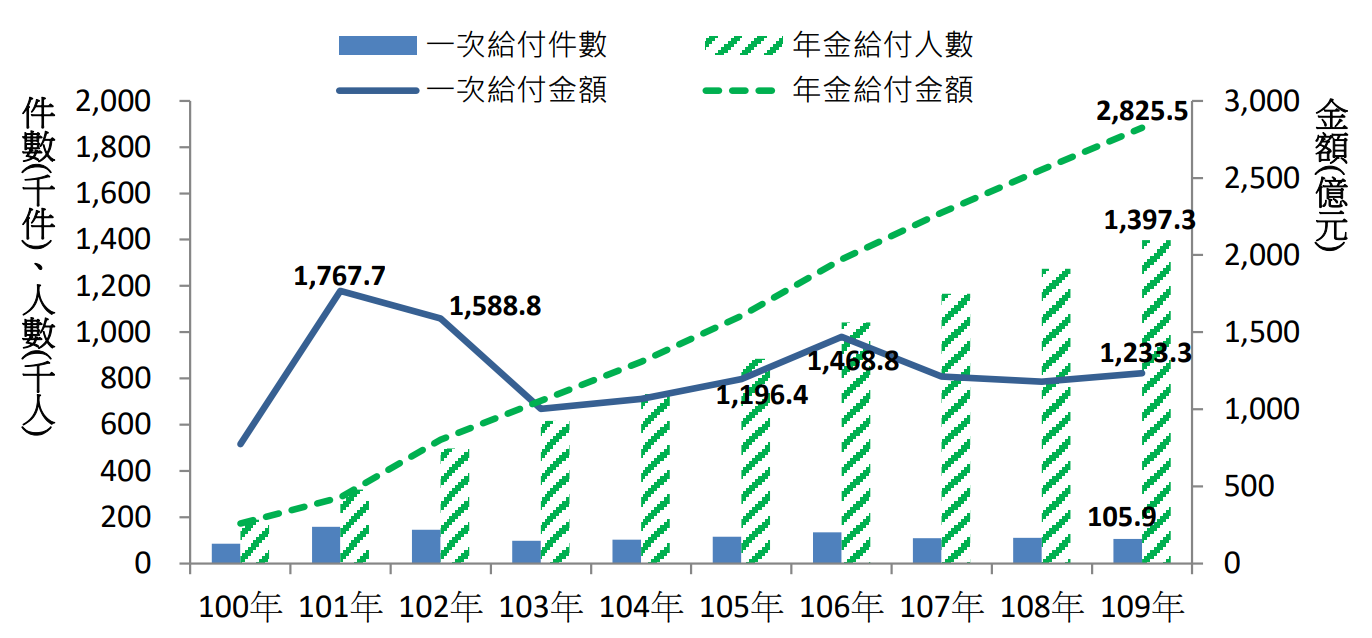
\includegraphics[width=0.8\textwidth]{tw_pension_pay.png}
    \caption{近10年勞保老年給付請領件數及金額(按一次給付及年金給付分)\protect\footnotemark}
\end{figure}
\footnotetext{圖片來源:\cite{old_age_econ5}}

從數據觀察,自年金化以來,年金請領件數及金額皆呈現穩定成長的趨勢,而一次給付則相對持
平。然而,在民國101年及105年時,一次請領人數明顯上升,兩次高峰皆延續約一年,可能正是
由於政府在此二時間點附近啟動年金改革相關計畫,並伴隨相關新聞,從而使一次請領人數明顯
上升。

自民國106年以來,勞保每年支出皆大於收入,根據107年的勞保基金精算結果,預估民國115年
勞保基金餘額將為負值。民國109年,台灣勞保的給付總額已然來到將近4.49兆元,其中老年給
付就佔了其中的90.4\%。在年金改革已是迫在眉睫的今日,年金改革對於勞動市場的影響仍是一個
未知數。

本計畫預計利用財政部財稅資料庫,透過建構異質性個人模型(heterogeneous agent model),
並將個人對於年金改革的信念加入模型之中,以探討年金改革對於勞動供給、儲蓄以及退休年齡等
勞動市場中重要變數之影響。特別地,本計畫將利用模型進行以下政策實驗:
\begin{enumerate}
    \item 比較民眾對於政府的信任程度不同時,對於年金改革的反應。
    \item 延長退休年齡。
    \item 減少退休金給付、延長平均月投保薪資計算期。
\end{enumerate}
以期預測年金改革對勞動市場之衝擊,並作為年金改革之參考。

\section*{\normalfont(三) 文獻回顧與探討}

自\cite{samuelson1958}證明了隨收隨付制(pay-as-you-go, PAYG)可能達成柏拉圖改善以來
\footnote{在一定的條件之下,詳見\cite{aaron1966}},年金制度一向是經濟學家研究的熱門
議題。過往的文獻依方法進行分類,大致可分為三類:縮減型模型(reduced-form model)、一般
均衡模型(general equilibrium model)以及單一個人模型(single agent model)。縮減型模型
的優點在於計算上相對容易,然而缺乏個體基礎使得其難以用於量化政策的影響或是擴充到同時
有多個退休金相關制度的情形,如台灣的勞工同時參加勞保以及勞退,即面臨此一困難。理想上,
一般均衡模型考慮了市場均衡,是最佳的研究形式,然而計算上的困難使得模型參數的選取經常
缺乏實證基礎。本計畫將採取第三種方法,即單一個人模型,忽略對於廠商的考量,考慮個人
的最佳決策,並利用財稅資料進行模型參數的估計。以下的文獻回顧將著眼於單一個人模型與過往
國內的文獻中對於勞動供給以及儲蓄的影響。

過往美國的研究經常聚焦在退休時間的特殊現象——大多數的退休時間集中在62及65歲。
\cite{burtless1986}與\cite{gustman1986}假設勞工可以無限制地借貸,並假設勞工有異
質的對休閒的偏好,成功地解釋了這個現象。社會安全年金(Social Security)在59到62歲,
每推遲一年退休可以增加終身年金給付725美元;62至65歲之間,每推遲一年退休可以增加807美
元的終身年金給付;若超過65歲,每晚一年退休則僅能增加536美元。這個特別的給付結構使得對
於休閒偏好較多的勞工在62歲時退休,而對於休閒偏好較少的勞工則在65歲時退休。

然而,\cite{rust1997}假設勞工完全不能借貸,同時也面對年金市場與醫療保險市場的運作不
完全限制。年金市場的運作不完全使得勞工僅能透過社會安全年金來跨期挪移所得,囿於社會安全
年金特殊的給付規則,勞工傾向於62歲時退休。然而,醫療保險市場的運作不完全使得部分勞工在
65歲前退休將會暴露在醫療支出的風險之中,這使得部分勞工選擇工作至65歲,直到被納入
Medicare的保險範圍。

\cite{french2005}考慮健康、工資的不確定性與遺產動機並假設勞工僅能持有正資產。研究發現
若移除對65歲以上的收入檢測制度\footnote{若收入超過一定水準,政府將會扣留一部份福利,美
國在2000年時移除對64歲以上年齡退休者的收入檢測。}(earnings test),平均退休年齡將延長一
年。此外,前述的借貸限制與社會安全年金結構的互動對勞動參與的影響則相對較小,若將提早退休
的年齡由62歲提高至65歲,對勞動參與幾乎沒有影響,因62歲時勞工通常擁有足夠的資產以應付多出
來的1年退休時間。同時,研究也進行了減少退休給付的實驗,發現減少年金給付20\%將會使平均退
休年齡延長3個月。

\cite{french2011}進一步考慮醫療保險Medicare的因素,利用某些雇主提供包含退休後的醫療
保險,有些則僅包含在職期間。研究發現,減少兩年的社會安全年金給付將使得60至69歲的人群工作
時間增加0.076年,而將Medicare的申請時間由65歲延後至67歲將使工作時間增加0.074年。另外,
研究也指出對於勞工而言,雇主所提供的醫療保險的價值有一半是來自於減少的醫療支出風險。同時,
對休閒偏好較強的個人傾向於工作於含退休後醫療保險的職位。

國內的研究就筆者所知,僅包括reduced-form model的研究或是一般均衡模型的研究。其中,
\cite{yang2009}利用人力運用調查資料,探討勞退新舊制變動對於工資的影響。結果顯示,整
體而言,在新舊制變動兩年內,整體而言薪資並未有顯著的變化。然而限縮在變動後才取得工作者
,其薪資顯著減少,且幅度大約為新制中雇主提撥額比例。\cite{yang2010}同樣利用人力運用調
查資料探討勞退新舊制對45至64歲之勞動供給的影響。結果顯示,勞動參與率在新舊制變動後顯著
下降,然而工時上升。\cite{chen2015}使用家庭收支調查資料並未發現勞保老年給付改革對於家
戶儲蓄率有顯著影響。

一般均衡的研究包括\cite{reform2017}所進行的包含公保、教保與勞保改革的研究。發現改革後
整體勞動雇用量下降。實質工資下降使得勞動供給下降,整體失業率上升。但該研究並未考慮不進行
改革所付出的成本,僅為改革前後的變化。另外,\cite{jhang2020}探討2018實行之公務人員年金
改革對總體經濟之影響。假定政府以定額稅融通公務人員退休金赤字,年金改革避免了在公務人員與
一般勞工間的所得重分配效果。研究發現,若同時實行延後退休年齡、以平均薪資計算退休金、降低
替代率之政策,公務人員將延後11年退休。

\section*{\normalfont(四) 研究方法及步驟}

\subsection*{\normalfont模型}
考慮追求終身效用極大的勞工$i$,其各期效用函數為CRRA,
\begin{equation}
    u_i(c,n) = \frac{1}{1-\gamma}(c^{\eta_i} (l-\theta_n n)^{1-\eta_i})^{1-\gamma}
\end{equation}
其中$c$為消費、$n$為勞動(假設$n$為離散,$n=1$為有工作;$n=0$則否)、$\theta_n$為工時、
$l-\theta_n n$為休閒、$1-\frac{1}{\eta_i}$為休閒對消費的替代彈性、$\gamma$為風險厭惡係
數。我們容許對休閒有異質的偏好,$\eta_i$服從有限的離散分布,參數為$\eta$。

工資$w_{it}$為
\begin{equation}
    \ln w_{it} = X_{it}\delta + f_i + \epsilon_{it}
\end{equation}
\begin{equation}
    \epsilon_{it} = \rho \epsilon_{i,t-1} + \xi_{it}, \xi_{it} \sim N(0,\sigma^2)
\end{equation}
其中$X_{it}$為個人的特徵如工作年數$h_{it}=h_{i,t-1} + n_{it}$、性別、教育程度等等,
$f_i$為固定效果。我們假設$\ln w_{it}$存在自相關,個人在$t$可觀察到$\epsilon_t$,但僅
知道$\xi_{i,t+1}$的分布。同時,勞工面對死亡風險$\mu_t$。假設為\cite{thatcher1999}所
提出的形式
\begin{equation}
    \mu_t = \frac{\theta_1}{1+ e^{\theta_2 - \theta_3 t}} + \theta_4
\end{equation}
$\theta_1,\theta_3 > 0$且假設存在壽命上限,$\theta_1+\theta_4 > 1$。

勞工面對的預算限制式為
\begin{equation}
    c_t + a_{t+1} = (1+r)a_t + w_t n_t + g(\pi_t,p_t)
\end{equation}
其中$a_t$為$t$期的期初資產、$r$為利率、$\pi_t$為$t$期初勞保累積保額、$p_t$為個人選
擇的退休金計畫($p_t=0$表示尚未領取)、$g(\cdot)$為年金給付之規則。

滿60歲後,勞工可以提領年金,若工作年資滿15年,則可選擇月退休金或一次請領;若工作年資
不滿15年,則只能一次請領。勞工必須在60歲至65歲間選擇退休計畫。

橫截條件(transversality condition)為
\begin{equation}
    \mathbb{E}_t[\frac{a_{T+1}}{(1+r)^T}] = 0
\end{equation}
其中$T$為該勞工死亡年齡。值得一提的是,無龐氏計謀條件(no-Ponzi scheme condition)
\begin{equation}
    \mathbb{E}_t[\frac{a_{T+1}}{(1+r)^T}] \geq 0
\end{equation}
在此模型中提供了自然的流動性限制,借貸限制會隨著年齡增加而緊縮。

另外,我們假設人們具有兩種信念(belief):一種相信年金有較高機率會進行改革\footnote{改革政策
包含延長退休年齡與減少給付等等不同情境,詳見政策實驗一節}($s_i=1$),另一種則較低
($s_i=0$)。每一期勞工認為年金在該期進行改革的機率$q_i$為
\begin{equation}
    q_i = q_0 + q_1 s_i + q_2\times reform_t + q_3\times s_i\times reform_t \text{, } s_i \sim Bernoulli(s)
\end{equation}
其中$reform_t$為該年度是否有年金改革之規劃,令$q=(q_0, q_1, q_2, q_3)$。

勞工有異質的時間偏好率$\beta_i$服從有限的離散分布,參數記作$\beta$。
最後,假設以上所有除$a_{40}, h_{40}, \pi_{40}$以外的隨機變數互相獨立。價值函數(value function)為
\begin{equation}
    \begin{split}
        &V_{it}(a_t,h_t,\pi_t,\epsilon_t,p_t,psr_t) = \\
        &\max_{c_t,n_t,a_{t+1},p_t} u_i(c_t,n_t) 
        + \beta_i (1-\mu_t) \mathbb{E}_t[V_{i,t+1}(a_{t+1},h_{t+1},\pi_{t+1},\epsilon_{t+1},p_{t+1},psr_{t+1})] \\
    \end{split}
\end{equation}
subject to
\begin{equation}
    c_t + a_{t+1} = (1+r)a_t + w_t n_t + g(\pi_t,p_t)
\end{equation}
\begin{equation}
    \pi_{t+1} = (1+r_p) \pi_t + \pi^f_t - g(\pi_t,p_t)
\end{equation}
\begin{equation}
    \mathbb{E}_t[\frac{a_{T+1}}{(1+r)^T}] = 0
\end{equation}
其中$\pi^f_t$為政府要求雇主每期付出的勞保費用,$psr_t$為政府是否實行年金改革($psr_t=1$
代表政府進行年金改革,0則否),$r_p$為勞保基金的利率。注意到模型為有限期的生命週期模型,
我們可以自模型終點向後求解。另外,因存在連續的狀態變數(state variable),我們將利用線性
插值進行近似。

\subsection*{\normalfont估計}
為了減輕計算的負擔,我們將採用兩階段的估計方法。第一階段,我們將利用最大
概似估計法(maximum likelihood estimation, MLE)估計死亡率的四個參數
$\theta_1,\theta_2,\theta_3,\theta_4$。另外,利用\cite{pistaferri2015}
的方法,我們得以將工資的參數$\delta,\rho,\sigma$獨立於主要模型的參數進行估計。第二階段
,我們將利用模擬動差估計法(simulated method of moments, SMM),選取目標動差以估計主模型
剩餘的參數。

在估計工資方程式
\begin{equation}
    \ln w_{it} = X_{it}\delta + f_i + \epsilon_{it}, \epsilon_{it} = \rho \epsilon_{i,t-1} + \xi_{it}, \xi_{it} \sim N(0,\sigma^2)
\end{equation}
時,我們首先面臨到的問題是$f_i$為觀察不到的固定效果,差分後可以得到
\begin{equation}\label{label:equation_wage}
    \Delta \ln w_{it} = \Delta X_{it}\delta - \rho \Delta X_{i,t-1} \delta + \rho \Delta \ln w_{i,t-1} + \Delta \xi_{it}
\end{equation}
,利用最小平方法估計$\delta$、$\rho$與$\sigma$。其次,我們僅能觀察到有工作的勞工的工
資,這會造成self-selection偏誤。仿照\cite{french2005}的方法,我們首先直接對有工作者估計
\ref{label:equation_wage}式,請注意這會高估平均工資。接著,將估計出的式子代回我們
主要的模型並模擬出所有勞工的潛在工資與勞動選擇。比較有工作者與全體的潛在工資,舉例來說,
若有工作者的薪資高於全體10\%,則將平均薪資調整為原先的90\%。最後,我們將調整後的平均薪資
再度代入主要模型之中。以上步驟重複至找到不動點為止。

另一項重要的估計問題是起始條件問題(initial condition problem),這主要源於模型中無法觀測
到的異質性,包括$s_i,\eta_i,\beta_i$。我們採用\cite{french2011}的方法,假設勞工為偏好
或信念$z_j$的機率為起始條件的logistic函數,其中$j$為偏好或信念的索引。最後,我們將利用SMM
估計主要模型的參數,包括各機率分布隨機變數的取值與機率。

\subsection*{\normalfont政策實驗}
\subsubsection*{\normalfont比較民眾對於政府的信任程度不同時,對於年金改革的反應}
在我們的模型之中,異質性$s$可以被視為是整體而言民眾對於政府的信任程度。我們將比較$s=0$
與$s=1$與估計之$s$所模擬出的各項所關心的變數,如勞動供給、儲蓄、退休年齡等等的差異。
\subsubsection*{\normalfont延長退休年齡}
我們將比較延長退休年齡對勞動供給、儲蓄、退休年齡等等的影響。其中,延長退休年齡的方式又
可分為兩種:一種是政府在某期宣布自該期起延長全民退休年齡1年;另一種則是政府在某期宣布自該
期起延長逐步退休年齡,每年以固定的速度延長,如每兩年上調一年等等。
\subsubsection*{\normalfont減少退休金給付}
我們將比較減少退休金給付20\%、50\%與100\%,對勞動供給、儲蓄、退休年齡的影響。另外,我們
也將考慮另一種改革方式,即針對國內現有「平均月投保薪資」的計算期間進行調整,包含延長至10年
、20年以及30年等等。

\section*{\normalfont(五) 預期結果}
如前所述,本計畫將建構一個異質性個人模型以預測民眾對於年金改革之反應。其次,透過利用模型
進行政策實驗,探討年金改革對於勞動供給、儲蓄以及退休年齡之影響,從而對年金改革提出建議。
\section*{\normalfont(六) 需要教授指導內容}
\begin{enumerate}
    \item 討論與理解現有文獻,並提出本計畫在文獻中的突破。
    \item 討論模型設定與推導,並完整掌握模型之經濟意義。
    \item 指導計量方法如EM Algorithm、initial conditions problem、
    identification problem等等以及如何加速程式計算。
    \item 指導論文寫作、編排等等。
\end{enumerate}

\bibliographystyle{apacite}
\bibliography{ref_res_app}
\end{CJK*}
\end{document}